\chapter{Operating system}\label{chap:os}


\marginnote{Frederik}

In the project description it is stated that a microprocessor shall run a user interface, a control system and SPI communication with the FPGA. This system will require the microprocessor to run multiple tasks and thus an operating system is necessary. It has been decided to use the provided microprocessor so the operating system has to be available for this system. The system has to run in real time to create a reliable environment for the regulation. Thus a real time OS was to be used.

It has been decided to use FreeRTOS both because it meets the requirements and is well documented, but also because the whole group has experience with FreeRTOS from the EMP course.

\section{ Pre-emptive Scheduling }


To ensure that the specific tasks is run in real time FreeRTOS use pre-emptive scheduling, this will be used. This is implemented by giving tasks priority when they are declared. Thus all tasks which have to run in real time is given a high priority. If a task is scheduled to run, but a task is already running, and the new task has a higher priority it can temporarily stop the task, run it's own task and resume the suspended task. That way a high priority task can be guaranteed to run at specific frequency or at certain interrupts. When every task has been set up, the function \texttt{vTaskStartScheduler()} will initiate the tasks and start an idle task to ensure that at least one tasks run.


\section{ Delays  }

For delays to occur in the system tasks does either need to be blocked by a timer or an i/o port. In FreeRTOS the time delay is handled by two different calls. To ensure that tasks run regularly each task is blocked with either \texttt{vTaskDelay} or \texttt{vTaskDelayUntil}. These calls will ensure a relatively or a precise frequency of operation respectively. \marginnote{Frederik} \texttt{vTaskDelayUntil} is able to do this by the user saving current tick at resume time and giving that as input to the function.
 
\section{ Semaphores }

To synchronize processes and avoid race conditions, FreeRTOS uses semaphores. The standard semaphore for synchronization between tasks is a binary semaphore. In FreeRTOS semaphores are created by, like with tasks, first creating a handler. Using the function \texttt{xSemaphoreHandle xSemaphore}

The FreeRTOS semaphore has two operations just like standard semaphores, the \texttt{wait()} and \texttt{signal()}. They are designed as \texttt{xSemaphoreTake} and \texttt{xSemaphoreGive}, respectively. The \texttt{xSemaphoreTake} checks if the semaphore is free and takes it if possible.
When obtained a semaphore can be released with \texttt{xSemaphoreGive}.

\section{ Queues }

In FreeRTOS queues are implemented as a method of intertask communication. It works as an FIFO buffer where the different tasks can either push or pop from the buffer.

\section{ Suspend }
It is also possible to suspend and resume tasks by function calls. If a task is suspended it will not get any CPU time regardless of it's priority.

%\section{Risks of faults}
%
%FreeRTOS does not do any work for error prevention. Does it is up to the developer %to 
%
%Is there a possibility of 
%Data corruption
%Deadlocks
%Priority inversion

\section{Inter task communication}\marginnote{Leon}
When multiple cooperating tasks run under the same system, some service must be
provided for sharing information and data. There are two ways of doing this. One
is to allow access to some shared memory and the other is to provide message
passing mechanisms.

The main difference between the to ways is that while message passing must be
provided by the operating system, shared memory is entirely up to the programmer
to control. In either case race conditions must be considered.

\subsection{Requirements}\marginnote{Leon du må lige uddybe}
In the considered pan-tilt system there are several paths requiring inter task
communication. By default the shared data must be protected by mutual exclusion
though it might be considered if data has to be reliable at all times. 

 It must be taken into consideration that some of the time critical tasks needs
 to access multiple parameters. For example the control task needs access to all
 system parameters to calculate the control signals.
 
 The inter task communication system should ensure low coupling to allow reuse
 of source code in other projects. It should also be considered, that the code
 might run on other operating systems so the coupling to the OS should also be kept
 low.
 
 Since multiple programmers will have to use the inter task communication
 system, it should be considered to uphold some similarity between the
 interfaces though different data structures lies behind.
 
 The system must provide interfaces for parameters, events, states, queues
and counters. Parameters will define the current state of the external system
thereby representing the entire interface to the physical system. States will be
used to control the state of the internal system state machine.

Events are used for presenting user inputs and timing events to the tasks and
are signified in the message being deleted once read. Counters are also simple
data structures and is in essence just another way of interfacing to a global
variable. The reason for maintaining counters as a separate interface is that
some systems provide hardware counters.

Though advanced queues are provided by FreeRTOS, a simple version is justified by
remaining a low coupling between the peripheral modules and the operating
system.

\subsection{Implementation}
The chosen solution is to build a simple common interface to shared memory. It
facilitates the simplicity of shared memory, while still retaining a low
coupling to the operating system. Another upside is that access to multiple
variables can be done under the same mutex, reducing overhead.

Seen from the calling application, variables are accessed by a function call.
Obtaining the mutex is done inside the function so instead of having a lot of
calls to the operating system sprinkled all over the source code, it is held in
one place. The interface function is based on a switch-case structure, ensuring
that as short time as possible is spend under the mutex.


\section{Memory management}\label{sec:memoryman}
%\section{Memory management}
This section discusses how memory is managed in the microcontroller. Programs for many embedded systems - especially ones with only a small amounts of memory available - only allocates memory to variables statically, before the program is executed. In the application written for the microcontroller in this project, most programmer-defined variables are static. Not all are, however, and the FreeRTOS kernel itself also uses dynamic memory allocation when creating new tasks, queues and the like. 


\subsection{Memory map}
The LM3S6965 microcontroller has 65 kB on-chip SRAM. That memory lies from address \texttt{0x20000000} to \texttt{0x20010000} \cite[71]{lm3s6965} and is where the data and BSS segments are contained. Additionally, the SRAM holds the stack and heap. Figure \ref{fig:memmap} displays a graphical representation of how the SRAM looks for a debug build. The data segment holds global and static variables that are explicitly initialized with a value. The BSS segment contains global or static variables which are uninitialized. The start-up code maps the data segment values from flash into SRAM and initializes the BSS area to zero.

\begin{figure}[htb]
	\centering
	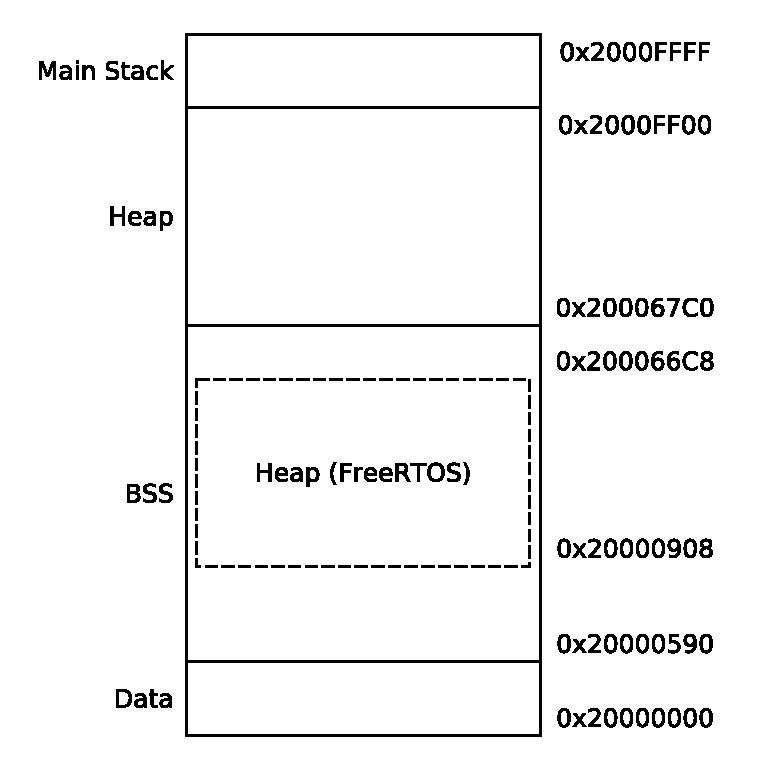
\includegraphics[scale=0.66,trim=0 0 0 0]{memorymap.pdf}%trim=l b r t
	\caption{Map of the SRAM for a debug build (commit \texttt{5e3d6c3e} on the Git tree).}
	\label{fig:memmap}
\end{figure}

Studying figure \ref{fig:memmap} one will notice that the heap used by FreeRTOS also resides in the BSS segment. This is because the FreeRTOS \texttt{heap\_2.c} memory allocation scheme declares the heap it uses as a large static array.

In the current implementation of the microcontroller application, both of the two heaps are used. At first only the FreeRTOS heap was defined, but along the way the need to use FreeRTOS' \texttt{vTaskGetRunTimeStats} function call arose. The function to print runtime statistics uses whatever \texttt{sprintf} function is available to generate formatted strings. On our system, using the GNU C Compiler to cross compile for the ARM Cortex-M3, \texttt{sprintf} is supplied by the Newlib C library implementation. The Newlib \texttt{sprintf} in turn uses Newlibs own \texttt{malloc} to dynamically allocate memory. This is where the second heap area comes in.

The second heap is quite simply two symbols defined in the linker script, marking the beginning and end of that memory area.


\subsection{Memory allocation schemes}
At the moment of writing, the microcontroller application uses both \texttt{pvPortMalloc} as implemented in \texttt{heap\_2.c} and \texttt{malloc} as it is implemented in Newlib. Here we'll take a short look at the two memory allocators and some of the differences between them.

The simplest of the two allocation schemes is FreeRTOS' \texttt{pvPortMalloc} (\texttt{heap\_2.c}). It works by dividing the static array, which it uses as heap, into smaller blocks. Initially the array is just one large block. When a call is made to \texttt{pvPortMalloc}, the large block is split. The size of the smaller blocks depends on how much memory is requested. Each memory block has a header which contains the size of that particular block and a pointer to the header of the next free block. The headers of the memory blocks form a linked list. When a memory allocation request is made, that linked list is traversed until a block of adequate size is found. Since the items in the linked list are sorted by the size of the memory block, the allocation algorithm is essentially a ``best fit'' algorithm. A call to \texttt{vPortFree} frees the memory block in question, but does not re-combine adjacent blocks. Nothing is done to prevent fragmentation, which allows a very fast way of freeing memory, but would cause problems if the application were to allocate and free blocks of unpredictable size.

The Newlib \texttt{malloc} implementation is more advanced. It is based on ``Doug Lea's Malloc'' \cite{dlmalloc}, which is widely used. The allocator will not be described in great detail here, as it would be beyond the scope of this report. However, some of it's main advantages and disadvantages, compared to the FreeRTOS \texttt{pvPortMalloc}, will be discussed.

The Newlib allocator allocates memory on the heap as \textit{chunks}, which is somewhat similar to what the FreeRTOS allocator does. There are some significant differences though: Unallocated chunks are grouped in \textit{bins} of fixed sizes. There are 128 bins in total. One of the main differences between the FreeRTOS and Newlib allocators is, that the Newlib allocator coalesces adjacent blocks, or chunks, of memory into one. They are then held in the bins, which are searched in size order. Special care is taken to improve efficiency, especially with regard to coalescing adjacent chunks of memory, by, for example, storing the size of the chunk both in the beginning and end of it.

As such, the FreeRTOS allocator is likely to be the fastest, but not necessarily the most efficient. It very much depends on the way the application works. If only memory blocks of fixed sizes are dynamically allocated, and the memory is not fragmented too much, the FreeRTOS allocator is probably the best, requiring the least overhead and being the fastest. On the other hand, if the size and order of memory requests are unpredictable, the Newlib allocator will most likely be better. Especially after the microcontroller has run for a long time, fragmentation could become a big problem and might render large parts of the memory unusable or at least increase search time to find free blocks.


\subsection{Use in this application}
In this application, the only time the Newlib allocator is used, is when generating runtime statistics through a call to \texttt{vTaskGetRunTimeStats}. This is in fact also the only place where allocations of unknown size could take place. All other allocations are memory for tasks, queues, SPI user buffers and UI menu items. These are of a known size, which can be determined with the \texttt{sizeof} operator at compile-time. The number and order of allocations is pre-determined.

There is a downside to using two heap areas and two allocator implementations though. If a memory area larger than the available space in \textit{one} of the heaps were to be requested, there would be no way of allocating it. Had there been one large heap instead, the request could have been successful. Using two allocator implementations also increases code size, which could be problem if the program had been so large, that there was no longer enough flash memory in the microcontroller.

\nomenclature{SRAM}{Static Random-Access Memory}


%\subsection{Discussion}
%A common way of sharing variables between tasks is to declare them globally.
%Then letting the individual tasks obtain a mutex and access the variable, either
%directly or by calling a function providing some interface to the variable.
%
%The upside of this solution is that it is easily implemented. The downside is
%increased coupling between different parts of the code, since multiple tasks are
%depending upon knowledge of both the operating system to obtain the mutex and
%the methods to access the variables.
%
%Another solution would be to rely only on the queues and semaphores provided by
%FreeRTOS. This resembles message passing, since the interface is provided by the
%operating system. The upside of this solution is, that coupling is now only
%between the task and the operating system and could be further reduced by using
%the preprocessor to provide a low coupling interface to any queue or semaphore
%in any operating system. The downside is a considerable amount of overhead,
%since the queue structure is a poor way of storing variables.

\section{Discussion}
The microprocessor could have used another scheduling than the pre-emptive
 provided by FreeRTOS. Though this would have made it harder to add new tasks, because a self but scheduler would not be as flexible.

A common way of sharing variables between tasks is to declare them globally.
Then letting the individual tasks obtain a mutex and access the variable, either
directly or by calling a function providing some interface to the variable.

The upside of this solution is that it is easily implemented. The downside is
increased coupling between different parts of the code, since multiple tasks are
depending upon knowledge of both the operating system to obtain the mutex and
the methods to access the variables.


Another solution would be to rely only on the queues and semaphores provided by
FreeRTOS. This resembles message passing, since the interface is provided by the
operating system. The upside of this solution is, that coupling is now only
between the task and the operating system and could be further reduced by using
the preprocessor to provide a low coupling interface to any queue or semaphore
in any operating system. The downside is a considerable amount of overhead,
since the queue structure is a poor way of storing variables.


\section{Implementation}
FreeRTOS was implemented and though it options was used extensively,
 some individual modules for memory management still had to be created. 
 The test which was performed, see \ref{sec:weq}, showed that the pre-emptive
 scheduling works well and that it is still possible to use more CPU time. 


The chosen solution for intertask communication is to build a simple common interface to shared memory. It
facilitates the simplicity of shared memory, while still retaining a low
coupling to the operating system. Another upside is that access to multiple
variables can be done under the same mutex, reducing overhead.


Seen from the calling application, variables are accessed by a function call.
Obtaining the mutex is done inside the function so instead of having a lot of
calls to the operating system sprinkled all over the source code, it is held in
one place. The interface function is based on a switch-case structure, ensuring
that as short time as possible is spend under the mutex.